\documentclass[12pt,a4paper]{scrartcl}
\usepackage[utf8]{inputenc}
\usepackage[T1]{fontenc}
\usepackage[french]{babel}
\usepackage{textcomp}
\usepackage{amsmath,amssymb}
\usepackage{lmodern}
\usepackage{graphicx}
\usepackage[dvipsnames,svgnames]{xcolor}
\usepackage{microtype}
\usepackage{hyperref}
\usepackage{lipsum}
\usepackage[pointedenum]{paralist}
\usepackage{listings}
\usepackage{graphicx}
\usepackage{multicol}
\usepackage{xspace}
\usepackage{xcolor}
\usepackage{amsthm}


\lstset{
language=python,
backgroundcolor=\color{Navy!10},
keywordstyle=\color{ForestGreen}\bfseries,
% numbers=left, numberstyle=\tiny,
tabsize=4,
}

\hypersetup{colorlinks=true,linkcolor=Brown,breaklinks=true,pdfstartview=XYZ}
\frenchsetup{StandardItemLabels=true}

\title{Équations différentielles}
\author{Gloria Faccanoni}
\date{15 janvier 2014}

\newcommand{\SNCF}{S.N.C.F}
\newcommand{\nompropre}[2]{#1~\textsc{#2}\xspace}
\newcommand{\nom}[2]{\textsc{#2}\xspace}

\theoremstyle{plain}
	\newtheorem{theoreme}{Théorème}[subsection]
	\newtheorem{proposition}[theoreme]{Proposition}
	\newtheorem{corollaire}[theoreme]{Corollaire}
	\newtheorem{definition}[theoreme]{Définition}
	\newtheorem{exo}{Exercice}


\begin{document}

\maketitle

\begin{abstract}
\lipsum[1][1-5]
\end{abstract}

\tableofcontents

\addsec{Introduction}
\lipsum[1-2]

\section{Rappels}
\label{eti}
\lipsum[3]

\subsection{Condition Initiale}
\lipsum[3]

\subsection{Problème de Cauchy}
\lipsum[4]

\section{Exercices}
\lipsum[7]

\section{Suite...}
On a vu dans la section~\ref{eti} page~\pageref{eti} les rappels nécessaire pour continuer la leçon.

\footnote
{A apprendre car vous êtes trop nuls}

\section{Entrainement sur les listes}
\begin{enumerate}
\item Ont des ailes
	\begin{enumerate}
	\item Volent
		\begin{enumerate}
		\item Hirondelle
		\item Aigle
		\item Ara
		\end{enumerate}
	\item Ne volent pas
		\begin{enumerate}
		\item Poule
		\item Autruche
		\end{enumerate}
	\end{enumerate}
	
\item Vivent dans la mer
	\begin{itemize}
	\item Respirent dans l'eau
		\begin{itemize}
		\item requin
		\item hippocampe
		\end{itemize}
	\item Respirent hors de l'eau
		\begin{itemize}
		\item Baleine
		\item Dauphin
		\end{itemize}
	\end{itemize}
	
\item Vivent sur terre
	\begin{description}
	\item[Australie:] kangourou, koala
	\item[Europe:] loup
	\end{description}	 
\end{enumerate}

\section{Code}

\lstinputlisting{src.py}

\section{Image}

Voici une image dans la marge, la voici en plus grand en figure~\ref{kruskal} \lipsum[2]

\marginpar{\fbox{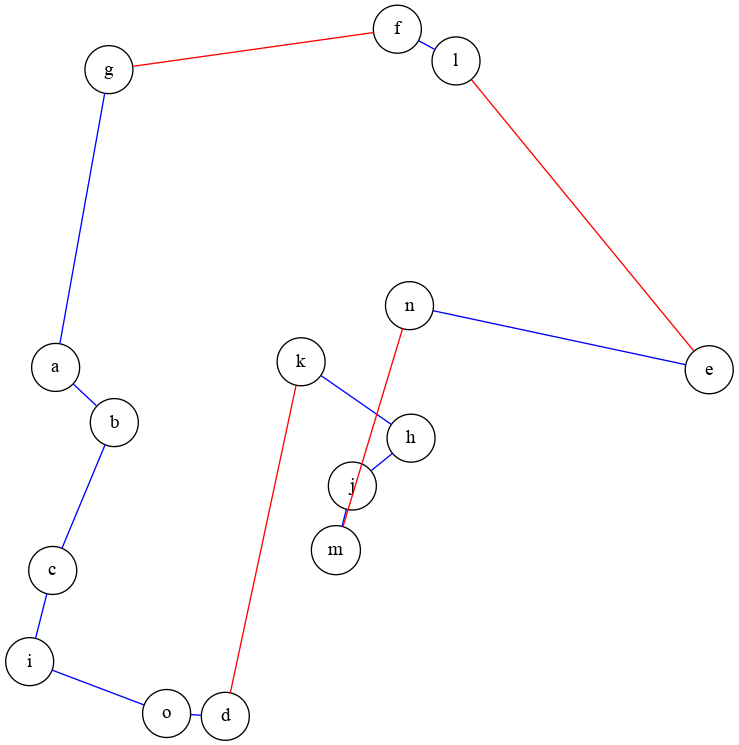
\includegraphics[width=1.7cm]{tsp}}}

\section{Image flottante}
\lipsum[3]
\begin{figure} % flottant
\centering
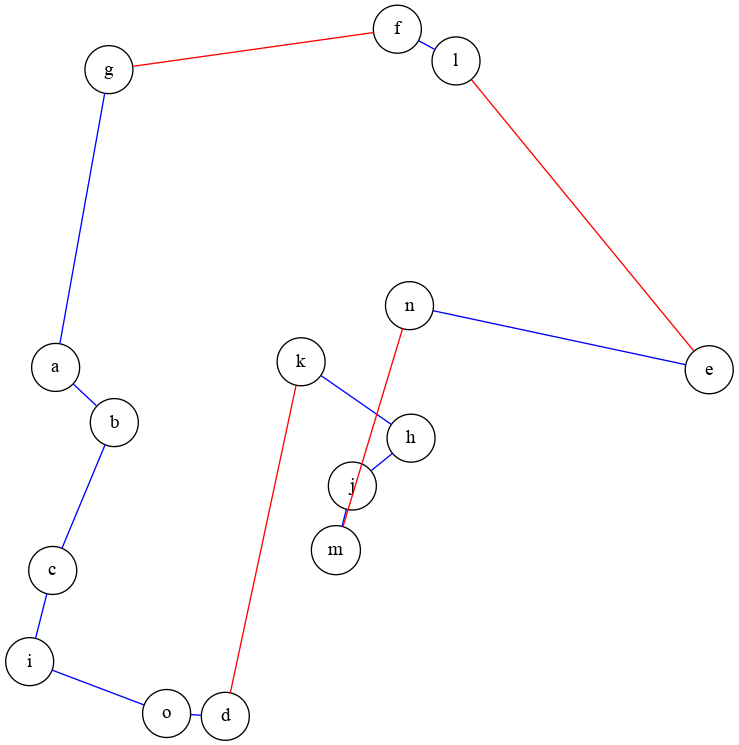
\includegraphics[width=10cm]{tsp}
\caption{Problème du voyageur du commerce avec l'algorithme de Kruskal}\label{kruskal}
\end{figure}
\lipsum

\section{Tableau}

Voici un tableau simple :

On peut se diriger sur le tableau \ref{tab1} :D !
Et hop c'est facile \lipsum[1]

\begin{table} % flottant
\centering

\begin{tabular}{|r|c|l|}
\hline
AA & BBB & C \\
\hline
D & EE & FFF \\ 
GGG & H & H \\
\hline
\end{tabular}

\caption{Le tableau de l'exemple}\label{tab1}

\end{table}

\section{Multicol}

\begin{multicols}{2}

\lipsum[3]

\columnbreak

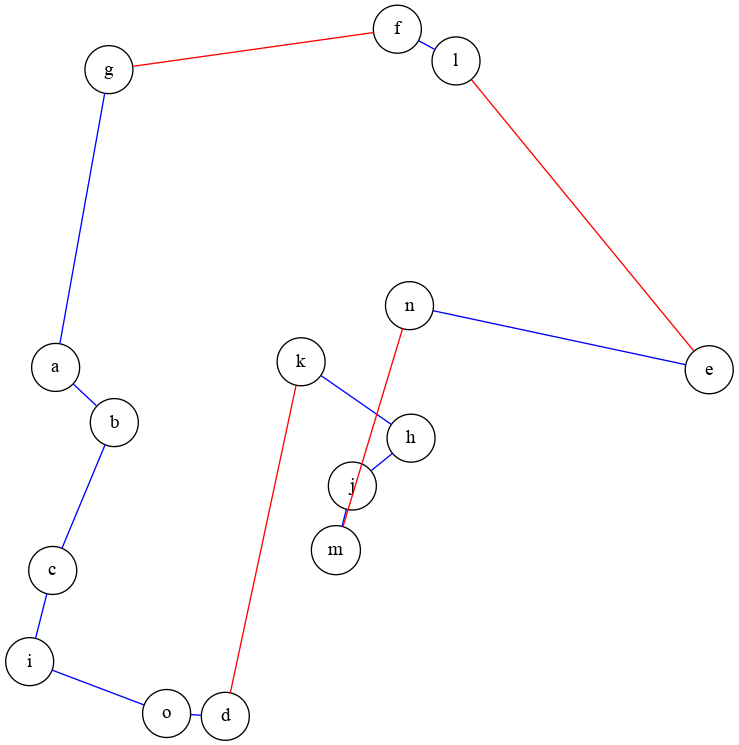
\includegraphics[scale=0.3]{tsp}
 
\end{multicols}

\section{Commandes / Macro}

\begin{itemize}
	
	\item \SNCF{} bla
	\item \SNCF bla
	\item \nompropre{Fabio}{Daussy}
	\item \nom{Fabio}{Daussy}	
	
\end{itemize}

\section{Mathématiques}

\subsection{Rappels}

\begin{definition}
Suspendisse vitae elit. Aliquam arcu neque, ornare in, ullamcorper quis, commodo eu, libero
\end{definition}

\begin{proposition}
Lorem ipsum dolor sit amet, consectetuer adipiscing elit. Ut purus
elit, vestibulum ut, placerat ac, adipiscing vitae, felis.
\end{proposition}

\begin{proof}
\lipsum[4]
\end{proof}

\begin{exo}
\lipsum[2][1-3]
\end{exo}

\begin{exo}
\lipsum[4][1-3]
\end{exo}



\subsection{Approfondissements}

\section{Formule}

Soit $f$ une fonction vérifiant

\begin{equation}
f(x)=2x+1
\end{equation}\label{eq.f1}

On a $f(x)-1=2x$ d'après~\eqref{eq.f1}

\begin{equation*}
	(x^2)^3 = x^{2^3}
\end{equation*}
\begin{equation*}
F_n = 7^{2^n}+1
\end{equation*}

$(x^2)^3$ et ${(x^2)}^3$ et $\left(x^2\right)^3$ et ${\left(x^2\right)}^3$

\begin{equation*}
	u_{n+1} = \sqrt[n]{1+u_n}
\end{equation*}
\begin{equation*}
	x_5 = \sqrt{1+\sqrt{2+\sqrt{3+\sqrt{4+\sqrt{5}}}}}
\end{equation*}

\begin{equation*}
 (\sqrt{x})^2 \text{ mais } \sqrt{x^2} \neq x \text{ en général }
\end{equation*}

\begin{equation*}
	y = x^2 \iff x = y^{1/2}
\end{equation*}

\begin{equation*}
	x > 0 \implies x^2 \neq 0
\end{equation*}

\begin{equation*}
	x \in X \setminus Y \implies x \not \in Y
\end{equation*}

\begin{equation*}
	x^{1/3} = x^{\frac{1}{3} = \sqrt[3]{x}}
\end{equation*}

\begin{equation*}
	\sqrt{2} = 1 + \frac{1}{2+\frac{1}{2+\frac{1}{2+\frac{1}{\ddots}}}}
\end{equation*}

\[
	\frac{\pi^2}{6}+\gamma = \Gamma(n) + \sqrt[n]{1+\alpha}
\]

\[
	cos^2(x) + sin^2(x) = 1
\]

\[
	2^{\ln(x)} = x^{\ln(2)}
\]

\[
	\sum_{n=1}^{+\infty}\frac{1}{n^2} = \frac{\pi^2}{6}
\]

\[
	\int_{0}^{1}-\frac{\ln(1-t)}{t}dt \approx 1,64493
\]

\[
\max_{ \substack{x,y \in E \\x \cdot y=0}}\varphi(x)
\]

\[
	\overrightarrow{OM} = \underbrace{O+\vec{u}}_{\text{point+vecteur}}
\]

\[
	\lVert x\rVert = 1 \iff \langle x,x \rangle = 1
\]

\[
	\lvert \{1,2,\dots,n\}\rvert = n
\]

\[
	\left\lfloor \sum_{n=1}^{N} u_n \right\rfloor^2 = N^2+N+1
\]

Soit $f : \mathbb{R} \to \mathbb{R}$ une fonction d’ensemble de définition $\mathcal{D}f$ et de courbe représentative $\mathcal{C}f$ .
Soit $\mathcal{F}$ une famille libre de vecteurs

\[
	\left.\begin{array}{c}
		a \in \mathbb{C} \\
		a \not \in \mathbb{R}
	\end{array}\right]
	\implies a \in \mathbb{C} \setminus \mathbb{R}
\]

\[
	\mathbb{M} = 
	\begin{pmatrix}
		m_{1,1} & \dots & m_{1,n} \\
		\vdots & \ddots & \vdots \\
		m_{n,1} & \dots & m_{n,n}
	\end{pmatrix}
\]

\begin{align}
	f:\mathbb{R}\to\mathbb{R} && g: \mathbb{R}\to\mathbb{R}\\
	x \to x^2 && x \to \sqrt{x}
\end{align}

\[
	\sqrt{\sum_{n=0}^{+\infty} u_n} 
	= 
	\left( \int_{a}^{b} f \mathrm{d} t\right) ^2 + \gamma \times \frac{\pi^2}{6}
\]


voir \cite{El03}


\bibliographystyle{plain}
\bibliography{biblio}

\end{document}




